%early draft, partly subsumed by CP_VG   ARM 3/4/16

\section{Games as a Recursive Data Type}

Chess, Checkers, Go, and Tic-Tac-Toe are examples of \emph{two-person
  terminating games of perfect information}---$\tg$'s for short.  These are
games where the move a player can make depends only on the visible board
position, or \emph{state} of the game.  ``Perfect information'' means that the
players know the complete state of the game at each move.  (Most card games are
\emph{not} games of perfect information because neither player can see the
other's hand.)  ``Terminating'' means that play cannot go on forever---it must
end after a finite number of moves.\footnote{Since board positions can repeat in
  chess and checkers, termination is enforced by rules that prevent any position
  from being repeated more than a fixed number of times.  So the ``state'' of
  these games is the board position \emph{plus} a record of how many times
  positions have been reached.}

We will define $\tg$'s \iffalse in a straightforward way tagged\fi as a 
recursive data type.  To see how this will work, let's use the game of
Tic-Tac-Toe as an example.

\subsection{Tic-Tac-Toe}
Tic-Tac-Toe is a game for young children.  There are two players who
alternately write the letters ``X'' and ``O'' in the empty boxes of a
$3 \times 3$ grid.  A grid pattern with three of the same letter
filling a row, column, or diagonal is called a \emph{tic-tac-toe}, and
the first player who gets a tic-tac-toe of their letter wins the game.
Children generally don't take long to figure out an optimal strategy
for playing the game.

We can diagram the ways to play Tic-Tac-Toe using a Tic-Tac-Toe game
tree.  The game tree starts with a \emph{root node} labelled with the
empty $3 \times 3$ grid.  This node then connects directly to
``child'' nodes labelled with each of the different grid patterns
possible after the first move.  According to Tic-Tac-Toe rules, the
X-player gets to move first, so the root of the tree connects directly
to nine different child nodes, each labelled with a different one of
the nine grid patterns containing one X and eight empty boxes.  Each
of these one-X child nodes connects in turn to eight child nodes of
its own labelled with the eight different one-X/one-O grid
patterns possible after the second player puts an O in a box.  These
move possibilities are given by the Tic-Tac-Toe \emph{game tree}
illustrated in Figure~\ref{fig:Tic-Tac-Toe}.

\begin{figure}
%\graphic{topgame}
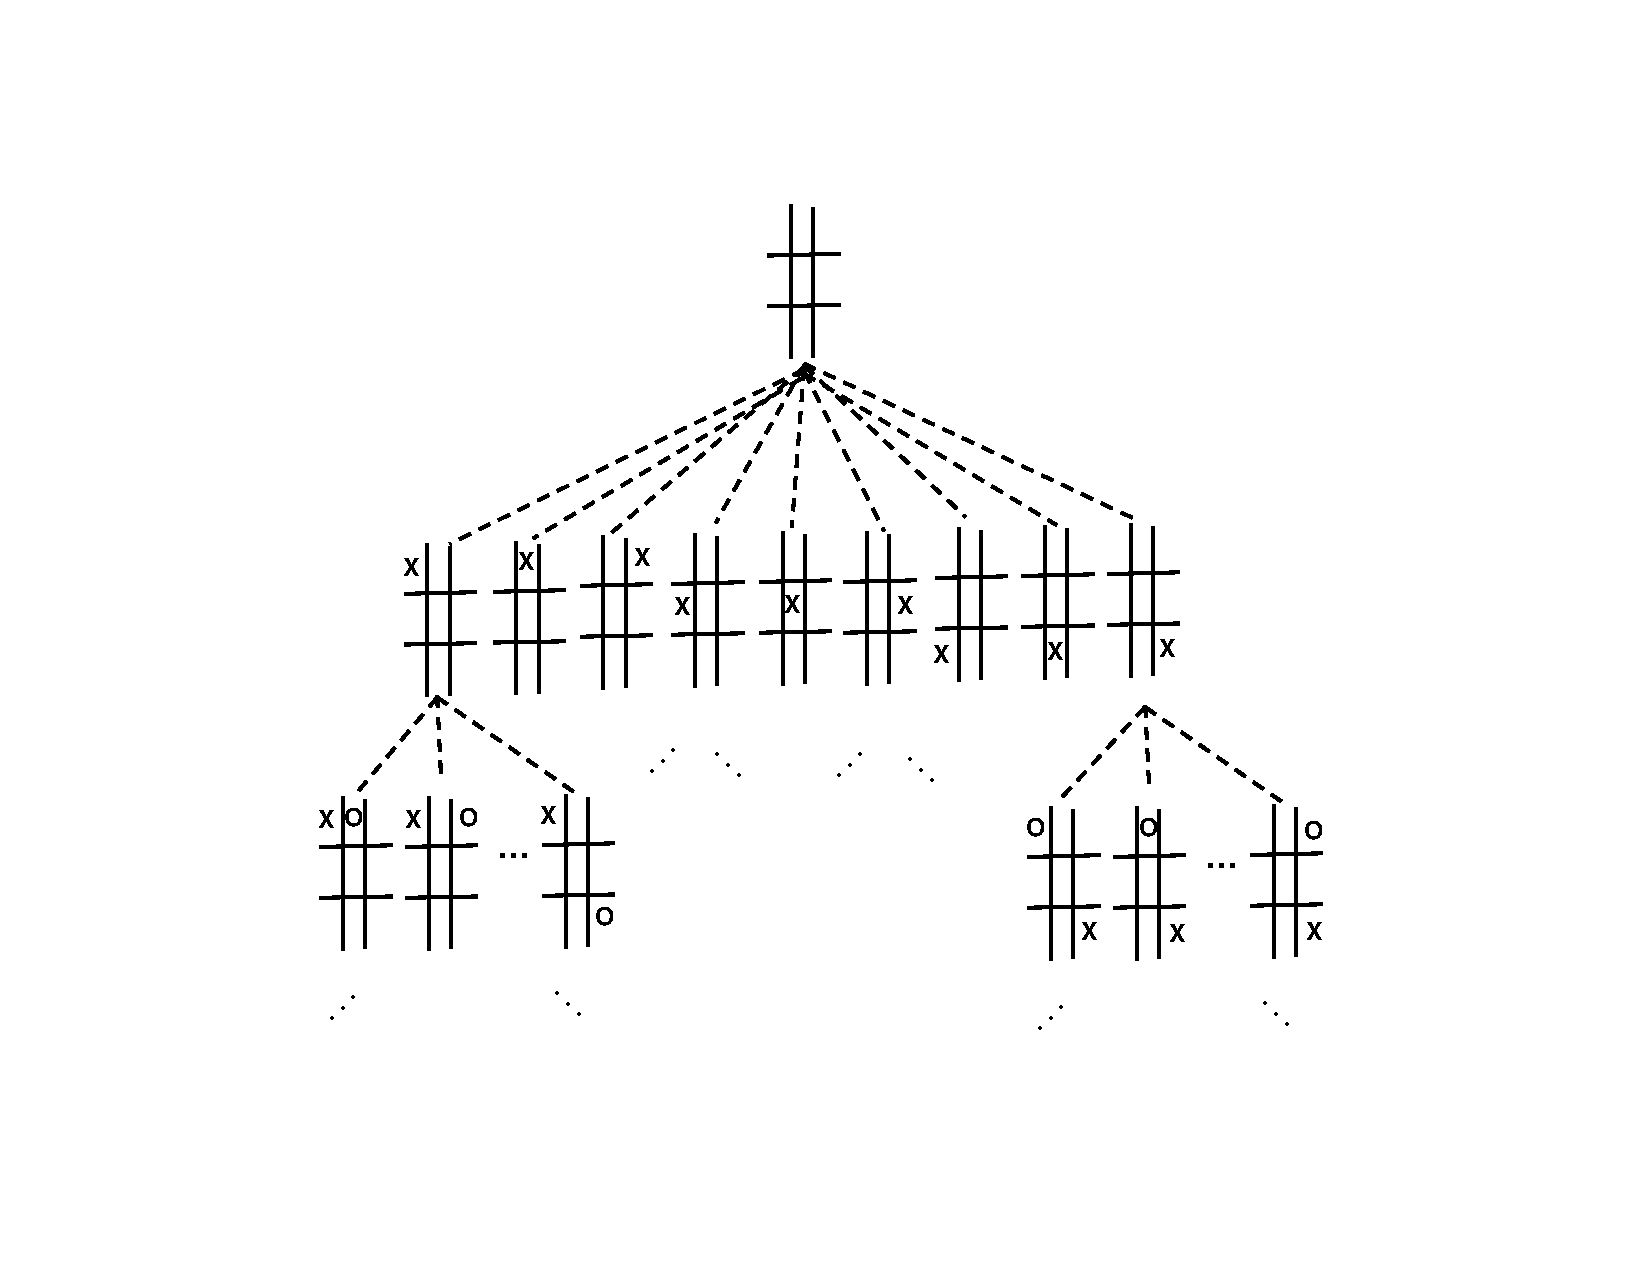
\includegraphics[width=6.5in]{topgame}
\caption{The Top of the Game Tree for Tic-Tac-Toe.}
\label{fig:Tic-Tac-Toe}
\end{figure}

The construction of the tree continues with each second move node
connecting to third level child nodes labelled with each of the seven
two-X, one-O patterns possible after the next move, and so on.  This
continues until all that's left are ``leaf'' nodes labelled with
\emph{terminated} patterns from which there is no further legal move.
The \term{terminated patterns} are those either containing a
three-in-a-row tic-tac-toe or else without any empty boxes.  (Quickie:
what is the highest level at which not every node has the the same
number of child nodes?)

The game tree embodies the rules and all the possible ways of playing
Tic-Tac-Toe.  It also illustrates another idea: each node in the tree
is the root of its tree of descendent of nodes.  This leads us to the
definition of the recursive data type of Tic-Tac-Toe trees.

\begin{definition}
The Tic-Tac-Toe game trees are defined recursively as follows:

\inductioncase{Base Case}: If $P$ is a terminated grid pattern, then a
single node labelled $P$ is a Tic-Tac-Toe tree.  This node is the root
of the tree and is also defined to be a \term{leaf} of the tree.

\inductioncase{Constructor case}: If $P$ is a non-terminated
Tic-Tac-Toe pattern, let $\mathcal{T}$ be a set of Tic-Tac-Toe game
trees whose roots are labelled with the distinct grid patterns
possible after one move from $P$.  Moreover, no node appears in
different trees in $\mathcal{T}$.  Then a tree with a root node not in
$\mathcal{T}$ and labelled $P$ whose child nodes are the roots of the
trees in $\mathcal{T}$, is a Tic-Tac-Toe game tree.  Its leaves are
the leaves of all the trees in $\mathcal{T}$.

\end{definition}

For example, for grid patterns
\begin{align*}
P_0 & =  \tbegin{array}{c|c|c}
                O & X & O\\
         \hline X & O & X\\
         \hline X & &
        \end{array}\\
Q_1 & = \begin{array}{c|c|c}
                O & X & O\\
         \hline X & O & X\\
         \hline X &  & O
        \end{array}\\
Q_2 & = \begin{array}{c|c|c}
                O & X & O\\
         \hline X & O & X\\
         \hline X & O & 
        \end{array}\\
R & = \begin{array}{c|c|c}
                O & X & O\\
         \hline X & O & X\\
         \hline X & O & X
        \end{array}
\end{align*}
a game tree with root labelled $P_0$ is pictured in Figure~\ref{fig:endgame}.

\begin{figure}[htbp]
%\graphic{endgame}
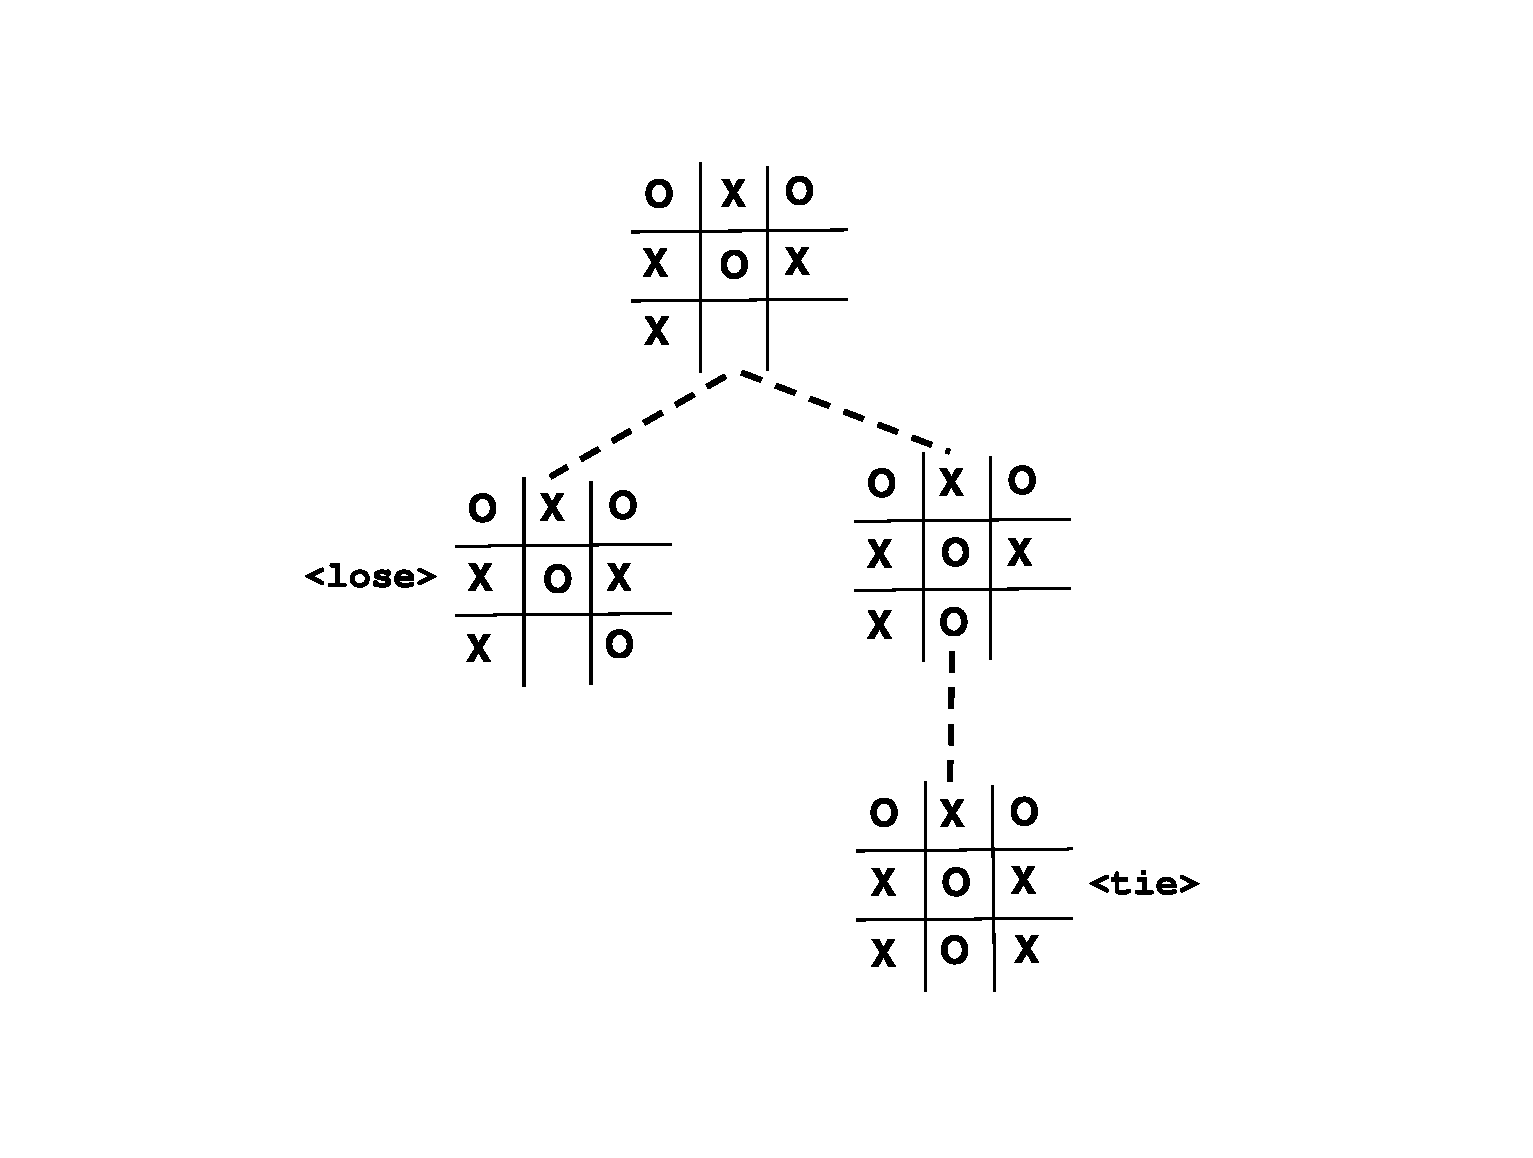
\includegraphics[width=6in]{endgame}
\caption{Game Tree for the Tic-Tac-Toe game starting at $P_0$.}
\label{fig:endgame}
\end{figure}

Game trees are usually pictured in this way, with the root at the top
and lines connecting down to children.  So the leaves appear at the
bottom of the tree---in Computer and geneaology, trees grow upside
down.  A path following connections down from the root to a leaf
describes a complete \term{play} of the game.

In English, ``Tic-Tac-Toe game'' might refer to the rules that define
Tic-Tac-Toe, the representation of those rules in the Tic-Tac-Toe game
tree whose root is labelled with an empty grid.  But ``Tic-Tac-Toe
game'' might also refer to a particular play, as in describing
yesterday's exciting Tic-Tac-Toe game.  It's usually easy to figure
out which way the phrase in being used, so we won't worry about this.

\begin{editingnotes}
\subsection{Infinite Tic-Tac-Toe Games}
At any point in a Tic-Tac-Toe game, there are at most nine possible
next patterns, and no play can continue for more than nine moves.  But
we can expand Tic-Tac-Toe into a larger game by running a 5-game
tournament: play Tic-Tac-Toe five times and the tournament winner is
the player who wins the most individual games.  A 5-game tournament
can run for as many as 45 moves.

It's not much of generalization to have an \emph{$n$-game Tic-Tac-Toe
  tournament}.  But then comes a generalization that sounds simple but can
be mind-boggling: consolidate all these different size tournaments into a
single game we can call \emph{Tournament-Tic-Tac-Toe ($T^4$)}.  The first
player in a game of $T^4$ chooses any integer $n > 0$.  Then the players
play an $n$-game tournament.  Now we can no longer say how long a $T^4$
play can take.  In fact, there are $T^4$ plays that last as long as you
might like: if you want a game that has a play with, say, nine billion
moves, just have the first player choose $n$ equal to one billion.  This
should make it clear the game tree for $T^4$ is infinite.

But still, it's clear that every possible $T^4$ play will stop.
That's because after the first player chooses a value for $n$, the
game can't continue for more than $9n$ moves.  So it's not possible to
keep playing forever even though the game tree is infinite.

This isn't very hard to understand, but there is an important
difference between any given $n$-game tournament and $T^4$: even
though every play of $T^4$ must come to an end, there is no longer any
initial bound on how many moves it might be before the game ends---a
play might end after 9 moves, or $9(2001)$ moves, or $9(10^{10}+1)$
moves.  It just can't continue forever.

While there is no bound on how long to play, at least after the
first move to an $n \times n$ board in meta-Tic-Tac-Toe, we know the game
will end with $n^2$ moves.

Now that we recognize $T^4$ as a \tg, we can go on to
a \emph{meta}-$T^4$ game, where the first player chooses a number,
$m>0$, of $T^4$ games to play, and then the second player gets the
first move in each of the individual $T^4$ games to be played.

Then, of course, there's meta-meta-$T^4$\dots.

Every play of the meta-meta game must still end, but now even
after the first move, there is no bound on how long a game might
continue.
\end{editingnotes}

\subsection{Two Person Terminating Games}

Familiar games like Tic-Tac-Toe, Checkers, and Chess can be assigned
scores of 1, -1, or 0 corresponding to win, lose, or draw.  The game of Go
is often scored by counting the difference in the numbers of locations
controlled by the two players.  An $n$-game tournament of win, lose draw
games might be scored by adding up the scores of the individual games,
which would equal the number of games won by the first player minus the
number they lost.  \iffalse A negative score would mean the second player
won more games.\fi

The idea behind the definition of $\tg$'s as a recursive data type is that
making a move in a $\tg$ leads to the start of a subgame, as in Tic-Tac-Toe.  So
given any set of games, we can make a new game whose first move is to pick a
game to play from the set.  At the end of play there is a score.

So what defines a game?  For Tic-Tac-Toe, we used the patterns and the
rules of Tic-Tac-Toe to determine the next patterns.  But once we have
a complete game tree, we don't really need the pattern labels: the
root of a game tree itself can play the role of a ``board position''
with its possible ``next positions'' determined by the roots of its
subtrees.  So any game is defined by its game tree.  This leads to the
following very simple---perhaps deceptively simple---general
definition.

\begin{definition}\label{tgdef}
  Let $S$ be a set of real numbers whose members will be called
  \emph{scores}. The \emph{game trees for $S$-scored two-person
    terminating games of perfect information} are defined recursively as
  follows:
\begin{itemize}

\item \inductioncase{Base case}:
\[
\ang{\textbf{leaf}, s} \in \tg,
\]
for all $s \in S$.

\item \inductioncase{Constructor case}:
If $\mathcal{G}$ is a nonempty set of
$\tg$'s, then $G$ is a $\tg$, where
\[
G \eqdef \ang{\textbf{tree},\mathcal{G}}.
\]
The game trees in $\mathcal{G}$ are called the possible \emph{next moves}
from $G$.
\end{itemize}

A \emph{play} of a $\tg$ $G$ is a (potentially infinite) sequence of
$\tg$'s starting with $G$ and such that if $G_1$ and $G_2$ are consecutive
$\tg$'s in the play, then $G_2$ is a possible next move of $G_1$.

If a $\tg$ has no infinite play, it is called a \emph{terminating} game.
\end{definition}

We already observed that even though the $T^4$ Tic-Tac-Toe tournament has
an infinite game tree, every play of $T^4$ must terminate.  We'll show
that this is true in general after we give a precise definition of
``play'':

\begin{theorem}
Every $\tg$ is terminating.
\end{theorem}

\begin{proof}
By structural induction on the definition of a $\tg$ $G$ with induction
hypothesis
\[
G \text{ is terminating}.
\]

\inductioncase{Base case}: If $G = \ang{\textbf{leaf}, s}$, then the only
possible play of $G$ is the length one sequence consisting of $G$ itself.
Hence $G$ terminates.

\inductioncase{Constructor case}: For $G = \ang{\textbf{tree},\mathcal{G}}$, we
must show that $G$ is terminating, given the structural induction
hypothesis that \emph{every} $G' \in \mathcal{G}$ is terminating.

Any play of $G$ is, by definition, a sequence starting with $G$ and
followed by a play starting with some $G_0 \in \mathcal{G}$.  But $G_0$ is
terminating, so the play starting at $G_0$ is finite, and hence so is the
play starting at $G$.

This completes the structural induction, proving that every \tg $G$ is
terminating.
\end{proof}



\subsection{Game Strategies}

A key question about a game is what strategy will give a player the best
score.  A \emph{strategy} for a player in a game specifies which move the
player should make at any point in the game.

In Tic-Tac-Toe for example, most elementary school children figure out
strategies for both players that each guarantees a score of 0, that is, a
draw.  Of course the first player can win if his opponent plays
childishly, but not if the second player follows the proper strategy.  In
more complicated games like Checkers or Chess, it's not clear what
strategy, if any, is guaranteed to yield the best score.
But structural induction makes it easy to prove that in any $\tg$,
both players have strategies that guarantee the best possible score.

In particular, there are two players called the \term{max-player} and the
\term{min-player} who alternate making moves.  The score measures what the
max-player wins (it might be negative, indicating that the min-player came
out ahead).  The objective of the max-player is to have play end with as
high a score as possible, while the min-player aims to end with as low a
score as possible.

\begin{editingnotes}
This could be simplified by having who moves first be defined by the
game itself.  Then a game has only one value, namely, the max value
that the max player can ensure---which equals the minimum value that
the min-player can hold down.
\end{editingnotes}

Given which of the players moves first in a game, a strategy for the
max-player is said to \emph{ensure} the payoff $s$ if play ends with a
score $ \ge k$, no matter what moves the min-player makes.  Likewise, a
strategy for the min-player is said to \emph{hold down} the score to $s$,
if play ends with a payoff of $\le s$, no matter what moves the max-player
makes.

A $\tg$ has two values: a \term{max value} and a \term{min value}.
The \emph{max value} is $s$ if the max-player has a strategy that
ensures payoff $s$, and the min-player has a strategy that holds down
the payoff to $s$, when the \emph{max-player moves first}.  Likewise,
the $\tg$ has \emph{min value} $s$, if the same thing holds when the
\emph{min-player moves first}.

The \emph{Fundamental Theorem} for 2-person 50-point games of perfect
information is that is that every game has both a max value and a min
value.  (Note: the two values are usually different.)

What this means is that there's no point in playing a game: if the max
player gets the first move, the min-player should just pay the max-player
the max value of the game without bothering to play (a negative payment
means the max-player is paying the min-player).  Likewise, if the
min-player gets the first move, the min-player should just pay the
max-player the min value of the game.

PPART\label{finpg} Prove this Fundamental Theorem for 50-valued
$\tg$'s by structural induction.

SOLUTION

The proof is by structural induction on the definition of a
  $\tg$ $G$.  The induction hypothesis is that there is that
\begin{quote}
  $G$ has a max value and a min value.
\end{quote}

\inductioncase{Base case}: [$G$ is the terminated game with payoff $k$].  The only
possible play is $k$.  So the max value and the min value are both $k$.

\inductioncase{Constructor case}: [$G = (G_0,\dots, G_n)$].  By structural
induction we may assume that each of the games $G_i$ have both max values
and min values.

We first show that $G$ has max value $k$ where $k$ is the largest min
value among the games $G_0,\dots,G_n$.

To prove the max value of $G$ is $k$, we must show how the max-player,
moving first in $G$, can ensure $k$, and how the min-player, moving second
in $G$, can hold down the payoff to $k$.

To ensure $k$, the max-player simply chooses $i$ as her first move where
game $G_i$ has this largest min value $k$.  The min-player then has the
first move in $G_i$, so by definition of min value, the max-player has a
strategy in $G_i$ that ensures $k$, which she can now follow.  So this
first move, combined with the ensuring strategy in $G_i$, defines a
strategy for the max-player in $G$ that ensures $k$.

Likewise, there is a simple strategy for the min-player, moving second in
$G$, to hold down the payoff to $k$.  Namely, suppose the max-player's
first move is $i$.  Then $G_i$ has a min value of $m \leq k$, since $k$ is
the largest min value.  So by definition of min value, there is a strategy
in $G_i$ for the min-player to hold down the payoff to $m$, which he can
now follow, thereby holding down the payoff of play on $G$ to $m \leq k$.

The existence of these ensuring and holding down strategies for $G$
implies that the max value of $G$ is $k$.

Second, to show that $G$ has a min value, we can repeat the previous
argument with min and max exchanged.

Therefore, by structural induction, we can conclude that all $\tg$'s have
min and max values.

SOLUTION

PPART A meta-$\tg$ game has as possible first moves the choice of
\emph{any} $\tg$ to play.  Meta-$\tg$ games aren't any harder to
understand than $\tg$'s, but there is one notable difference, they
have an infinite number of possible first moves.  We could also define
meta-meta-$\tg$'s in which the first move was a choice of any
$\tg$ \emph{or} the meta-$\tg$ game to play.  In
meta-meta-$\tg$'s there are an infinite number of possible first
\emph{and} second moves.  And then there's $\text{meta}^3-\tg$ \dots.

\iffalse
The 2D-origin game in a Week 4 class problem is a game in which there are
an infinite number of possible first moves, an infinite number of possible
second moves, \dots.  \iffalse (with two values, ``win'' or ``lose''
instead of values from -50 to 50)\fi
\fi

To model such infinite games, we could have modified the recursive
definition of $\tg$'s to allow first moves that choose any one of an
infinite sequence
\[
G_0,G_1,\dots,G_n,G_{n+1}, \dots
\]
of $\tg$'s.  Now a $\tg$ can be a mind-bendingly infinite datum
instead of a finite one.

Do these infinite $\tg$'s still have max and min values?  In
particular, do you think it would be correct to use structural induction
as in part~\eqref{finpg} to prove a Fundamental Theorem for such infinite
$\tg$'s?  Offer an answer to this question, and briefly indicate why
you believe in it.

SOLUTION

It may not be obvious, but structural induction is a perfectly sound proof
technique even for infinite recursively defined data, and the proof of the
Fundamental Theorem for $\tg$'s applies without change to infinite ones.

SOLUTION

\begin{theorem}\label{fund}
  \textbf{Fundamental Theorem for Two-Person Games:} For every two-person
  terminating game of perfect information, has a max-value and a
  min-value.
\end{theorem}

\begin{proof}
The proof is by structural induction on the definition of a $\tg$ $G$.
The induction hypothesis is that there is a winning strategy for $G$.

\inductioncase{Base cases}:
\begin{enumerate}

\item $G=\ang{\textbf{leaf}, \textbf{win}}$.  Then the first player has the
 winning strategy: ``make the winning move.''

\item $G=\ang{\textbf{leaf}, \textbf{lose}}$.  Then the second player has a
 winning strategy: ``Let the first player make the losing move.''
\end{enumerate}

\inductioncase{Constructor case}: Suppose $G = \ang{\textbf{tree},\mathcal{G}}$.
By structural induction, we may assume that some player has a winning
strategy for each $G' \in \mathcal{G}$.  There are two cases to consider:
\begin{itemize}
\item some $G_0 \in \mathcal{G}$ has a winning strategy for its second
  player.  Then the first player in $G$ has a winning strategy: make the
  move to $G_0$ and then follow the second player's winning strategy in
  $G_0$.

\item every $G' \in \mathcal{G}$ has a winning strategy for its first
  player.  Then the second player in $G$ has a winning strategy: if the
  first player's move in $G$ is to $G_0 \in \mathcal{G}$, then follow the
  winning strategy for the first player in $G_0$.
\end{itemize}
So in any case, one of the players has a winning strategy for $G$, which
completes the proof of the constructor case.

It follows by structural induction that there is a winning strategy for
every $\tg$ $G$.
\end{proof}

Notice that although Theorem~\ref{fund} guarantees a winning strategy, its
proof gives no clue which player has it.  For the Subset Takeaway Game of
Problem~\ref{CP_subset_take_away} and most familiar $\tg$'s like Chess,
Go, \dots, no one knows which player has a winning
strategy.\footnote{Checkers used to be in this list, but there has been a
  recent announcement that each player has a strategy that forces a tie.
  (reference TBA)}

%% Games as a Recursive Data Type Problems %%%%%%%%%%%%%%%%%%%%%%%%%%%%%%%%%%%%
\begin{problems}
\practiceproblems
\pinput{TP_Game_trees}
\end{problems}

\end{editingnotes}
